\documentclass[a4paper,12pt]{article}


\pagenumbering{arabic}

\NeedsTeXFormat{LaTeX2e}
\usepackage{url}
\usepackage{listings}
\usepackage{fancyhdr}
\usepackage{amsmath}
%\usepackage{prelim2e}
% \usepackage{draftcopy}
\usepackage{pdfpages} 
\usepackage{graphicx}
\usepackage[pdftitle={Reporte - Doctorado},pdfauthor = {Alfredo Ortega},pdfsubject={Reportes y avances de investigación de spread-spectrum sobre fibra óptica},colorlinks=true,linkcolor={blue}]{hyperref}
\usepackage[spanish]{babel}
\usepackage[utf8]{inputenc}
\usepackage{pst-eps,graphicx,epstopdf}
\pagestyle{fancy}

\title{Reporte Doctorado}
\author{Alfredo A. Ortega }
\date{\today}


\begin{document}
 
\begin{titlepage}
\null\vfill
\begin{center}\Large
Reporte de Doctorado
\par
\small \textit{Avances sobre investigación sobre Spread Spectrum} \par
\vskip1cm
\small Alfredo Ortega\par
Instituto Tecnológico de Buenos Aires\par
\vskip1cm
Febrero 2008
\end{center}\vfill

\begin{abstract}
En este artículo se documentan los avances sobre la investigación sobre spread-spectrum como parte del Doctorado en Informática.
El foco de la tesis es implementar un esquema criptograficamente seguro a nivel de link (OSI Capa 2) en enlaces de fibra óptica.
\end{abstract}

\end{titlepage}

\author{Alfredo Ortega}

\tableofcontents

\section{Introducción}
En el 2007 durantes los cursos del doctorado, se comenzó a explorar la posibilidad de implementar un esquema de spread spectrum sobre fibra óptica.
Spread Spectrum es un técnica utilizada exitosamente en muchos protocolos de comunicaciones modernas, tales como Bluetooth, Wifi, etc.
Básicamente se expande el espectro de la señal a transmitir utilizando una segunda señal conocida. 
La modificación puede ser en tiempo, frecuencia, o modulación directa. Esto conlleva una disminución de la eficiencia de la transmisión, pero una señal con espectro expandido tiene muchas otras ventajas, como por ejemplo la coexistencia con otra señal (o ruido) de banda estrecha.

\section{Ruido en canal simetrico binario}

\begin{figure}[t]
  \begin{center}
    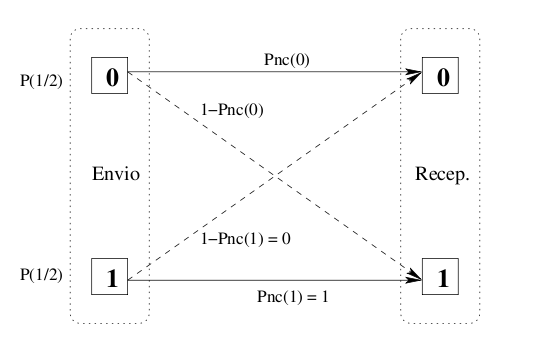
\includegraphics[scale=0.43]{canalBinario.png}
  \end{center}
\caption {Canal binario: esquema de probabilidad}
\label{fig:canbin}
\end{figure}

Para calcular el ruido en un canal simétrico binario, calculamos la probabilidad de no-colision que tendra un usuario determinado, ya que las colisiones seran el ruido del canal (En esta etapa no consideramos otros tipos de ruido que pueda tener el canal físico).

\noindent Cantidad de slots por trama: $m$
\noindent Cantidad de usuarios: $n$

\noindent Probabilidad de no colisión para un usuario en un canal simétrico:
\begin{equation}
P_{nc}=\left(\frac{m-1}{m}\right)^{n-1}
\end{equation}


\noindent Probabilidad de no colisión para un usuario en un canal óptico:
\begin{eqnarray}
P_{nc} & = & P(1) \cdot P_{nc}(1) + P(0) \cdot P_{nc}(0) \\
P_{nc} & = & \frac{1}{2} \cdot 1 +  \frac{1}{2} \cdot \sum_{i=0}^{n-1} 
C^{n-1}_{i} \left(\frac{m-1}{m}\right)^i  \left(\frac{1}{m}\right)^{n-1-i}  \left(\frac{1}{2}\right)^{n-1-i} 
\end{eqnarray}

\noindent Donde $\left(\frac{m-1}{m}\right)^i$ es la probabilidad de no
colisión de $i$ canales (se suma para todo posible número de canales no
colisionando: $1\leq i\leq n$, que están en otro slot), $
\left(\frac{1}{m}\right)^{n-1-i}$ es la probilidad de colisión de los restantes
$n-1-i$ (estos están en el mismo slot que el canal actual, el `$-1$' es para no
contar el canal actual), y la colisión se produce cuando los otros canales
transmiten $1$ cuya probabilidad es $\left(\frac{1}{2}\right)^{n-1-i}$. El
factor $C^{n-1}_{i}$ suma sobre todas las combinaciones posibles de canales no
colisionando, que son hechos independientes.

\noindent Teniendo en cuenta que $ \sum_{i=0}^{n-1}
C^{n-1}_{i} \left(\frac{m-1}{m}\right)^i  \left(\frac{1}{2m}\right)^{n-1-i}$ es la potencia $n-1$ de un binomio, reemplanzando tenemos
\begin{eqnarray}
P_{nc} & = & \frac{1}{2} +  \frac{1}{2} \cdot \left(\frac{m-1}{m} + \frac{1}{2m} \right)^{n-1} \\
P_{nc} & = & \frac{1}{2} +  \frac{1}{2} \cdot \left(1- \frac{1}{2m} \right)^{n-1} \\
P_{nc} & \simeq & \frac{1}{2} +  \frac{1}{2} \cdot e^{-1/2} 
\end{eqnarray}

\noindent Donde la última aproximación vale para $n=m$ y $n$ grande.


\vspace{5mm}

\noindent Para el caso de {\em bloom} filters con $k$ filtros\footnote{Se envían $k$ repeticiones del bit en canales distintos, entonces basta que sólo uno de ellos sea 0 para que recibamos un 0 en un canal óptico.} la probabilidad de no colisión es:
\begin{eqnarray} 
P_{nc}^{k} & = &  P(1) \cdot P_{nc}^{k}(1) + P(0) \cdot P_{nc}^{k}(0)\\ \label{Pnc_k}
\end{eqnarray}
Sabiendo que la probabilidad de no colisión para el 0 es:
\begin{eqnarray}
P_{nc}^{k}(0) & = & 1 - \big(P_{c^k}(0)\big)^k 
\end{eqnarray}
Pero la probabilidad de colisión para el 0 cuando se transmiten $k$ copias es:
\begin{eqnarray}
P_{c^k}(0) & = & 1 - \big(P_{nc^k}(0)\big)  \enspace,
\end{eqnarray}
y que además la probabilidad de no colisión para los $k$ slots del bloom
filter es
\begin{eqnarray}
P(\mbox{no col.} k) &=& P(\mbox{no col.}1)\cdot P(\mbox{no col.}2)\cdot P(\mbox{no col.}3)\cdots P(\mbox{no col.}k)\\
&=&\left(\frac{m-1}{m}\right)\cdot\left(\frac{m-2}{m-1}\right)\cdot\left(\frac{m-3}{m-2}\right)\cdots\left(\frac{m-k}{m-(k-1)}\right)\\
&=& \frac{m-k}{m} \enspace.
\end{eqnarray}
Luego la probabilidad de colisión con alguno de las $k$ copias del bit es
\begin{eqnarray}
P(\mbox{col.}k)&=& 1-P(\mbox{no col.} k)\\
&=& 1-\frac{m-k}{m}\\
&=& \frac{k}{m} \enspace.
\end{eqnarray}
Entonces reemplazamos y calculamos:
\begin{eqnarray}
P_{c^k}(0) & = & 1 - \left(\sum_{i=0}^{n-1} C^{n-1}_{i} \left(\frac{m-k}{m}\right)^i \left(\frac{k}{2m}\right)^{n-1-i} \right)  \\
& = &  1-\left( 1-\frac{k}{2m}\right)^{n-1}
\end{eqnarray}
Reemplazando esta ecuación en~\ref{Pnc_k} obtenemos:
\begin{eqnarray}
P_{nc}^k & = & \frac{1}{2} + \frac{1}{2} \left( 1- \left( 1- \left( 1- \frac{k}{2m} \right)^{n-1}  \right)^{k}  \right) 
\end{eqnarray}

Sin embargo, este calculo es incorrecto, comparandolo con los datos que da el simulador. La formula entrega valores de error menores con respecto a los reales, como se observa en la figura. 
Los trazos del mismo color corresponden a el mismo K con azul(K=1), verde (K=2) y rojo(K=4). M=256


%\begin{figure}[th]
%  \begin{center}
%    \includegraphics[scale=0.7]{comparacion}
%  \end{center}
%  \caption{Error de calculo}
%  \label{fig:Gal}
%\end{figure}


\section{Entropia}

Comenzemos por lo básico:

Segun Shannon, el \textbf{contenido de informacion} h(x) de un suceso x dada la posibilidad que suceda P(x) es:
$$ h(x) = log_{2}\left(\frac{1}{P(x)}\right) $$

Y la entropia de un conjunto A, H(A) se define simplemente como el promedio del contenido de información:

$$ H(A) = \sum_{x E A_{x}} P(x)log_{2}\left(\frac{1}{P(x)}\right)$$

En un canal binario solo dos sucesos existen, uno con probabilidad p, y otro con probabilidad 1-p, por lo tanto para p siendo la probabilidad de error:

$$ H(p) = -p log_{2}(p)-(1-p)log_{2}(1-p) $$

\section{Entropia condicional}

Vamos a analizar la entropia de dos conjuntos X de entrada y Y de salida interrelacionados.

La entropia condicional de X dado $y=b_k$ donde $b_k$ es un valor dado, es la entropia de la distribucion de probabilidad $P(x|y=b_{k})$:
$$H(X|y=b_{k}) = \sum_{x \in A_{x}} P(x | y=b_{k})\log_2\left(\frac{1}{P(x | y=b_{k})}\right) $$

La entropia codicional de X dado Y es el promedio, sobre y, de la entropia condicional de X dado y:
$$H(X|Y) =  \sum_{xy \in A_{x}A_{y}} P(x,y)\log_2\left(\frac{1}{P(x,y)}\right) $$

\section{Información mútua}
La información mútua entre X e Y es:
$$I(X;Y) = H(X)-H(X|Y)$$
Mide el promedio de reduccion de la incertidumbre acerca de x que resulta de saber el valor de y, o viceversa: la cantidad promedio de informacion que x revela acerca de y.

\section{Capacidad de canal}

La capacidad C de un canal discreto sin memoria es :

\begin{equation}
C = \max_{{\cal{P}}_x} I(X;Y) 
\end{equation}

O sea, la máxima información mutua entre los alfabetos X de entrada e Y de salida.
Para hallar el maximo podemos derivar $I(X;Y)$ con respecto a la probabilidad $P_x$.
Para un canal binario asimétrico sin memoria con probabilidad de error $p$, la capacidad máxima $C$ es:

\begin{equation}\label{Cap}
C = 1 - H(p) 
\end{equation}

Si expandimos H(p) en \ref{Cap}:

$$ c = 1-\left(p \times \log_2\left(\frac{1}{p}\right) + (1-p) \cdot \log_2\left(\frac{1}{1-p}\right)\right) $$
Simplificada:
$$ c = 1 + p * \log_2(p) + (1 - p) * \log_2(1-p) $$

Sin embargo esta capacidad es menor que la que realmente tenemos en nuestro canal, ya que un Z-channel se adecua mayormente a los medios de transmision opticos.

\section{Z-channel}

Un canal Z (Z-channel) difiere de un canal binario, ya que las probabilidades de bit-flip son asimetricas.
Los Z-channel se usan generalmente para modelar sistemas de transmision opticos.

\begin{figure}[th]
  \begin{center}
    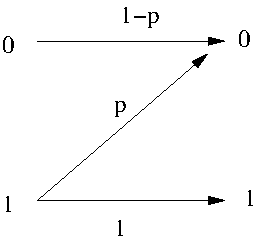
\includegraphics[scale=0.5]{zchannel}
  \end{center}
  \caption{Diagrama: Z-channel}
  \label{fig:Gal}
\end{figure}

Para un Z-channel, la distribucion de probabilidades de I(X;Y) es diferente, por lo que obtenemos un máximo diferente:

$$ C_{Z} = 1 - \left(\frac{1}{2}*H(p)\right) $$ \cite{tallini}

Por lo tanto,

$$ C_{Z} = \log_2\left(1+(1-p) p^{p/(1-p)}\right) $$


\begin{figure}[th]
  \begin{center}
    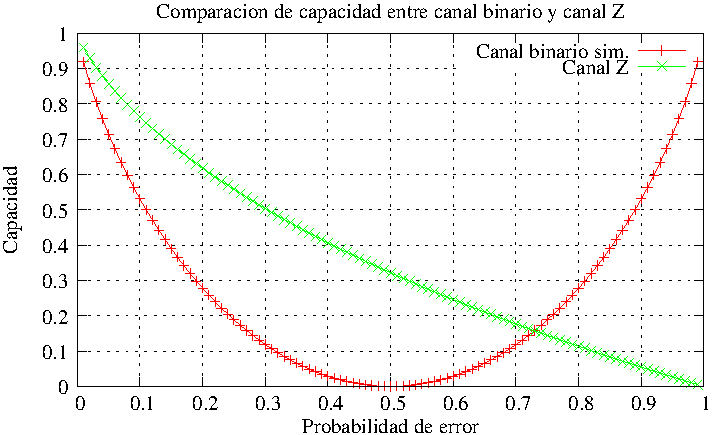
\includegraphics[scale=0.9]{comparacionBZ}
  \end{center}
  \caption{Diagrama: Azul: Capacidad de canal binario Verde: Capacidad de canal Z}
  \label{fig:CompBZ}
\end{figure}

\section{Parámetro de seguridad}
(De Cryptograpy by V. V. IAshchenko)\cite{primes}

Primero, para el análisis de complejidad de un sistema criptográfico se suele utilizar un parametro variable que mide el tamaño del problema y representa a la vez los requerimientos del algoritmo criptográfico tanto como la probabilidad de un adversario de romper la seguridad en el sistema, Este es el llamado parametro de seguridad, por ejemplo esto puede ser el largo de clave.
Este parámetro puede tomar valores arbitrariamente grandes.
Segundo, la definición de seguridad depende de la tarea que el adversario trata de realizar y de la informacion acerca del esquema criptográfico disponible.
Tercero, se debe especificar el valor en el cual la cantidad de calculos necesarios por el atacante se presumen irrealizables, esto sera funcion del parametro de seguridad.
Segun la thesis de Edmond, el algoritmo del atacante se considera eficiente si esta limitado en tiempo polinomial sobra la longitud de la entrada (el parametro de seguridad en este caso) de otra manera se considera infeasible.
Notese que el algoritmo criptografico mismo debe ser eficiente.

Finalmente se debe fijar un limite para la probabilidad negligible. El contrato criptografico estandard dice trata a la probabilidad como negligible si no excede $\frac{1}{p(n)}$  para un polinomio $p$ y el parametro de seguridad $n$.

Aceptadas esas cuatro definiciones, para probar que un algoritmo criptografico es seguro basta con probar que la no-existencia de un algoritmo polinomial que realize la tarea del adversario.

De todas maneras, el estado actual de la teoria de complejidad no permite justificar un limite inferior de un problema como super-polinomial ($P=NP?$) por lo que todas las pruebas en el mundo de la seguridad estan basadas en asumciones no probadas.
Por lo tanto, la investigacion se concentra usualmente en buscar las condiciones suficientes mas debiles (o necesarios y suficientes) para la existencia de un esquema seguro.
Las asumciones son usualmente generales (Basadas en la teoria de complejidad) o basadas en intratabilidad de problemas en la teoria de numeros, etc.

\subsection{algoritmo1}

Se estudiara el parámetro de seguridad para el algoritmo 1:

Este algoritmo consta de $r$ clientes cada uno con una serie de $n$ posiciones pre-seleccionados.
La cantidad posible de combinaciones de $n$ posiciones es de $ _{n}P_{r} = \frac{n!}{(n-r)!} $.
Definimos que el algoritmo se rompe cuando un atacante puede inferir la serie de posiciones $n$ para un cliente.

Existe un algorimto de selección de $n$ que suponemos no posee ninguna debilidad, o sea, elije $r$ conjuntos de $n$ posiciones tal que teniendo una, no se pueda inferir otra.
Un algoritmo sencillo que cumple estas características es una simple búsqueda exaustiva. No es óptima en tiempo pero cumple con las características de seguridad requeridas.

Suponemos:
\begin{itemize}
 \item El algoritmo de selección no tiene debilidades.
 \item El atacante no posee control de los datos a transmitir, y estos son totalmente randomizados.
\end{itemize}

Dadas estas suposiciones (Equivalen a un ataque con plain-text desconocido en jerga criptográfica) para inferir el conjunto de posiciones $n$ de un cliente, el atacante debera probar exaustivamente todo el conjunto de $ _{n}P_{r}$ sobre una trama capturada, y ese sera el parámetro de seguridad, hasta que demostremos lo contrario.

\section{mediciones}

A continuación expondremos algunos graficos resultados de las simulaciones. La figura \ref{capacidad} muestra la capacidad teórica máxima de un canal binario frente a otro canal Z, con respecto aumentan los clientes en un frame de 256 clientes.

\begin{figure}[th]
  \begin{center}
    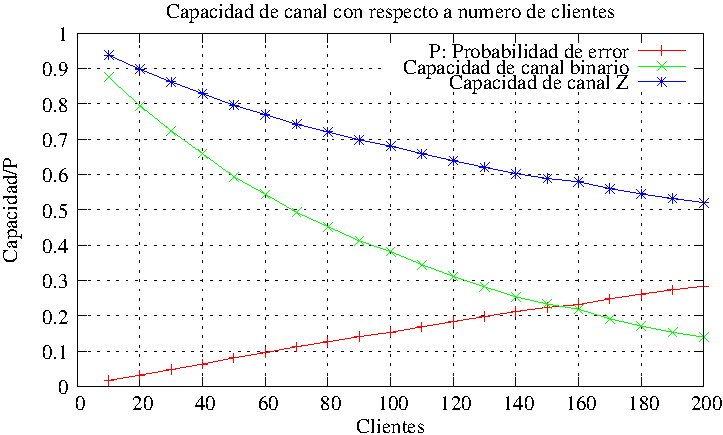
\includegraphics[scale=1.0]{capacidad1}
  \end{center}
  \caption{Comparacion de capacidad: Binario (Verde) Z-channel (Rojo)}
  \label{fig:capacidad}
\end{figure}

Sobre este sistema, se corrieron varias simulaciones, y la figura  \ref{comparacioncapacidad} muestra dos lineas, que representan el error de algoritmos LDPC+Reed-Solomon y Reed-Solomon puro. El punto en el que las curvas se elevan de cero, marca la capacidad maxima del algoritmo, que puede contrastarse con la capacidad maxima teórica.

\begin{figure}[th]
  \begin{center}
    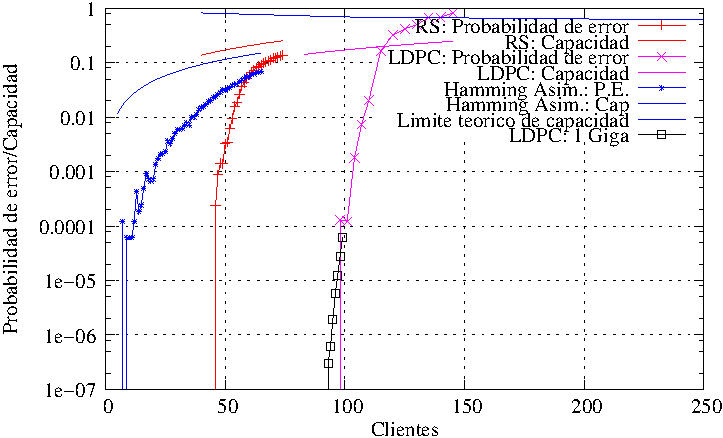
\includegraphics[scale=1.0]{comparacion_rs_ldpc}
  \end{center}
  \caption{Simulaciones: LDPC y Reed-Solomon contra capacidad teórica}
  \label{fig:comparacioncapacidad}
\end{figure}


\bibliographystyle{plain}	% (uses file "plain.bst")
\bibliography{myrefs}		% expects file "myrefs.bib"


\end{document}
